%%%%%%%%%%%%%%%%%%%%%%%%%%%%%%%%%%%%%%%%%%%%%%%%%%%%%%%%%%%%%%%%%%%%%%%%%%%%%%%
% Itroduccion
%%%%%%%%%%%%%%%%%%%%%%%%%%%%%%%%%%%%%%%%%%%%%%%%%%%%%%%%%%%%%%%%%%%%%%%%%%%%%%%

\chapter{Introduction}

The first years of proton-proton collisions at a centre of mass energy of 7 TeV delivered by
the Large Hadron Collider and recorded by the ATLAS experiment have provided data to
explore quantum chromodynamics (QCD) at scales never reached before. Precision measurements of strong interactions are interesting in their own right, but, in addition, QCD provides one of the main
backgrounds to many New Physics measurements; furthermore, it is also through tests of QCD
that New Physics may be discovered. Hadronic jets are a fundamental ingredient for precision
tests of QCD: understanding and measuring their performance is crucial in the LHC environment. %This thesis presents....


%\section{Introduction}\label{sec:introduction}

A wide range of physics signatures, within the Standard Model predictions (SM) and Beyond the Standard Model (BSM), contain jets originating from bottom ($b$) quarks. 
%Within the SM a range of production channels exist for heavy-quark jets, $\eg$ pure QCD production or in association with heavy bosons ($W, Z, H$). Furthermore, $b$-quarks enter in many collider searches, notably because they are produced in the decays of various SM particles, \eg top quarks and the Higgs boson, and of numerous particles appearing in proposed extensions of the SM. 
The ability to identify jets containing $b$-hadrons\footnote{Due to QCD confinement the experimental signature of quarks and gluons are not the quarks and gluons themselves but a spray of ``colorless'' hadrons. In the case of the $b$-quarks, the so called $b$-hadrons are observed.} is therefore important for the high-$\pt$ physics program of the ATLAS experiment. $b$-tagging algorithms rely on the relatively long decay length of $b$-hadrons that gives rise to large impact parameter tracks and displaced decay secondary vertices; or on the presence of a soft lepton within the jet, the product of the semileptonic $b$-decay.   
%Two robust $b$-tagging algorithms taking advantage of either the impact parameter of tracks~\cite{ATLAS-CONF-2010-091} or the reconstruction of secondary vertices~\cite{ATLAS-CONF-2010-042} were developed and successfully used for several analyses of the 2010 and 2011 data. Building on this experience, more advanced and performing $b$-tagging algorithms have been recently commissioned with 2011 data~\cite{ATLAS-CONF-2011-102}.
%The more advanced taggers %are based on Monte Carlo predictions for the signal ($b$-jet) or background (light- or $c$-jet) hypotheses and
%use multivariate techniques %such as likelihood ratios and neural networks 
%to further increase the discrimination between $b$-jets and light jets.
These algorithms, however, do not provide information on the number of $b$-hadrons within the jet. In particular, they tag jets containing a $b\bar{b}$ pair, with no net heavy flavour, which do not correspond to the intuitive picture of a
$b$-jet as a jet containing a single $b$-quark or antiquark.
%In particular they tag gluon jets if they give rise to a close-by $b$-hadron pair via gluon splitting. 
%, as depicted in Fig.~\ref{fig:gbbcartoon}. 

%We will henceforth call ``merged'' $b$-jets %$b \bar{b}$  the
 $b$-jets containing two $b$-hadrons, henceforth called ``merged'',  and single $b$-jet, the jets containing only one $b$-hadron, are depicted in Fig.~\ref{fig:gbbcartoon}. 

%The ability to single out merged $b$-jets expected to be produced in QCD mainly by gluon splitting,  has several applications. 

% in different lines of analysis: measurement of QCD beauty production, $t\bar{t}$ and single top production, reduction of background in searches with $b$-quarks in the final state, and the study of substructure in fat jets, where merged $b\bar{b}$ jets from QCD compete with boosted $Z\rightarrow b\bar{b}$ and $H\rightarrow b\bar{b}$ jets.
\begin{figure}[h]
\centering
%\includegraphics[width=0.25\textwidth]{FIGS/Single_b_fix.png}
%\hspace{1cm}
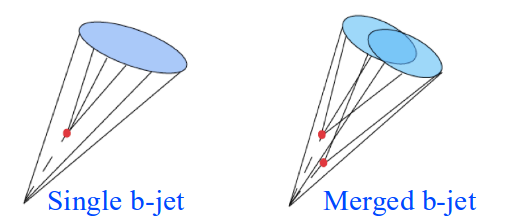
\includegraphics[width=0.8\textwidth]{FIGS/Single_b_Merged_bb.png}
\caption{$b$-tagging algorithms select jets originating both from the fragmentation of single $b$-quark (``single'' $b$-jet, left image) or from the splitting of a gluon into a pair of close-by $b \bar{b}$ quarks (``merged'' $b$-jets, right image).}
\label{fig:gbbcartoon}
\end{figure}
% \caption{$b$-tagging algorithms select jets originating both from the fragmentation of single $b$-quark (``single'' $b$-jet, left image) or from the splitting of a gluon into a pair of close-by $b$-hadrons (``merged'' $b$-jets, right image).}
%\caption{A $b$-jet can originate from the fragmentation of single $b$-quark (``single'' $b$-jet, left image) or from the fragmentation  of a pair of close-by $b$-quarks
%splitting of a gluon into a pair of close-by $b$-hadrons(``merged'' $b$-jets, right image).}



%------------------------------------------------------------------------
%\section{Physics Motivation}\label{sec:motivation}
%------------------------------------------------------------------------
%Reduced version
%In this section we briefly discuss two applications of the study and indentification of merged $b$-jets: the measurement of QCD $b$-quark production and the reduction of background in SM and Beyond the Standard Model (BSM) analyses.

The ability to single out merged $b$-jets expected to be produced in QCD mainly by gluon splitting,  has several applications.
% The ability to distinguish genuine $b$-quark jets from those produced via gluon splitting is thus of wide application.
 %Here we briefly discuss three cases, the measurement of QCD $b$ quark production, the reduction of background in SM and BSM analyses with $b$ quarks in the final state, and studies of jet substructure.%
%
Here we briefly discuss two cases, the measurement of QCD $b$-quark production and the reduction of background in SM and Beyond the Standard Model (BSM) analyses.


\\[5mm]
{\em The measurement of the inclusive $b$-jet spectrum}

% We have not followed Marcel's suggestion to substantially shorten the inclusive b-jet spectrum subsection to give true credit to the measurement suggestion that motivated our development: a b-jet xsection that excludes double-B jets. Here is a new version where we try to make it clearer the line of thought that led to this proposal
%a. Full NLO calculation of the inclusive b-jet spectrum yields a K-factor=6-10.
%b. Herwig analysis shows that FEX and GSP contributions are much larger than FCR. This is due to strong enhancement from collinear logarithms.
%Proposal: move to inclusive flavour-kt b-jet xsection where bb-jets are not counted. Theoretical uncertainties are substantially reduced
%a. Flavour-kt b-jet xsection is free of final-state (GSP) logarithms
%b. Initial-state (FEX) collinear logarithms can be resummed if one uses a b-quark PDF



Studies of QCD bottom production are important because of the correspondence between parton level production and the observed hadron level, and their potential to provide information on the $b$-quark parton distribution function, a component of the proton structure thought to be generated entirely perturbatively from the QCD evolution equations of the other flavours. The theoretical calculation of the inclusive $b$-jet spectrum presents rather important uncertainties ($\sim 50\%$), considerably larger than those for the light jet inclusive spectrum ($\sim 10-20\%$)~\cite{Frixione:1996nh}. These arise from the poor convergence of the perturbative series, as evidenced by the large value of the $K$-factor (NLO/LO), $K$ = 6 -- 10, in the $\pt$ range covered by the LHC. While at LO only the so-called ``flavour creation'' channel is present, at NLO two new channels open up, often referred to as ``flavour excitation'' (FEX) and ``gluon splitting'' (GSP), see Fig.~\ref{fig:qcd_diagrams}. NLO effects are included approximately in LO parton showering models, such as {\sc Herwig}
%~\cite{Herwig} 
or {\sc Pythia}.
%~\cite{PYTHIA6}. 
The various channels can be approximately separated in a parton shower Monte Carlo generator such as these, where one can determine the underlying hard process from the event record. It is found that the LO channel has a much smaller contribution than 
%the two channels that at fixed order enter only at NLO because these 
the FEX and the GSP channels, which
receive strong enhancement from collinear logarithms~\cite{GSP}. 

%Fig.~\ref{fig:qcd_diagrams} shows examples of diagrams at LO (``flavor creation''), where the $b$ and $\bar{b}$ quarks fly in opposite directions, and at NLO (``gluon splitting'', GSP), where a gluon splits collinearly into a close-by $b\bar{b}$-pair that the clustering algorithm classifies within the same jet. A jet containing both $b$ and $\bar{b}$ is considered to be a plain $b$-jet in standard definitions.
%The largest uncertainties are associated to the GSP contribution, that receives a strong enhancement from collinear logarithms. 
%This channel however does not even correspond to one's physical idea of a $b$-jet, \ie the one induced by a hard $b$-quark, and it seems somehow unnatural to include it at all as part of one's $b$-jet spectrum. 

Ref.~\cite{Salam.AccurateHQ} proposes a new observable to free the heavy-flavour spectrum calculation from collinear logarithms, and improve the accuracy of the theoretical prediction,
%for improving the accuracy of the prediction of the heavy-flavour spectrum 
by not including in the production cross-section the contribution from double $b$-hadron jets. Final-state logarithms are removed by employing a recently developed jet reconstruction scheme, the flavour-$k_t$ algorithm~\cite{flavorkt}, which maintains the correspondence between partonic flavour and jet flavour. Specifically, jets containing a $b$-quark and a $b$-antiquark, which in a parton shower MC generator are produced $\sim95\%$ of the time by the GSP channel, are labeled in an IR-safe way as light jets and removed from the $b$-jet spectrum.
The initial-state (FEX) collinear logarithms can be resummed by using a $b$-quark parton distribution functions.
With this algorithm the $K$-factor for the differential heavy-jet spectrum cross-section is shown not to exceed a value of $K=1.4$, with a factor of four reduction in the theoretical (scale variation) uncertainties.
%
\begin{figure}[h!]
\centering
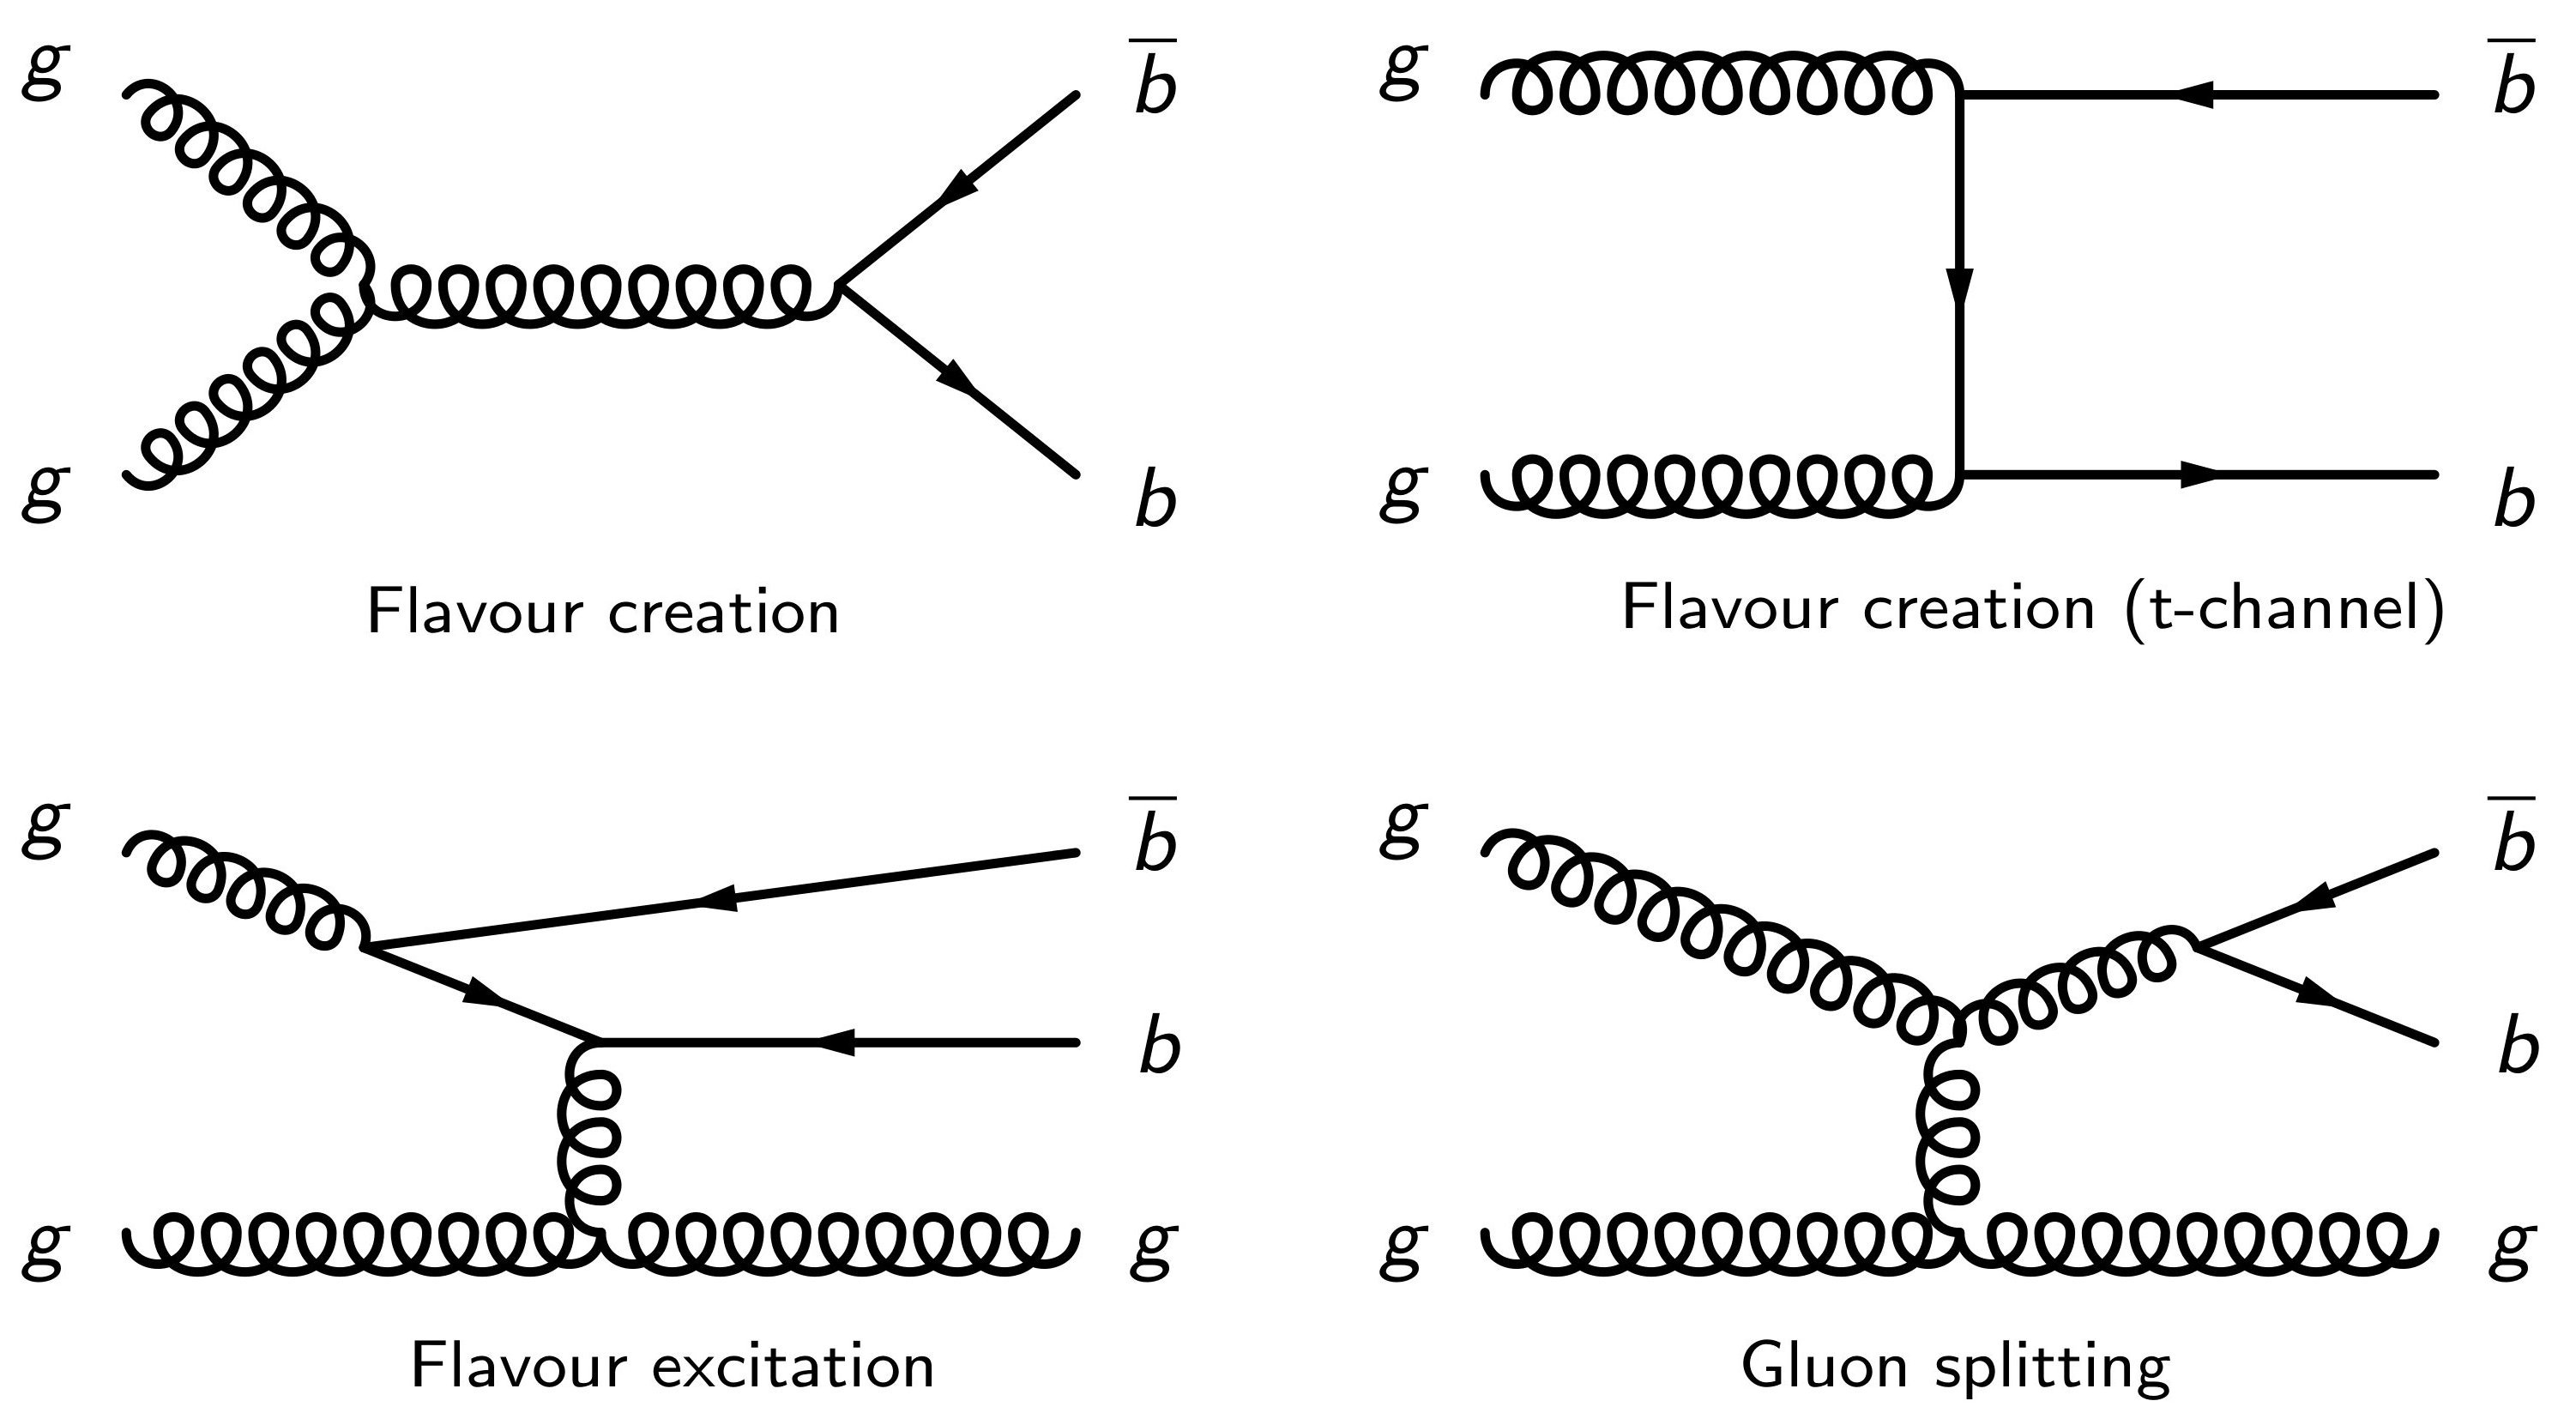
\includegraphics[width=0.32\textwidth,viewport=0 880 1500 1600,clip]{FIGS/bb_diagrams.jpg}
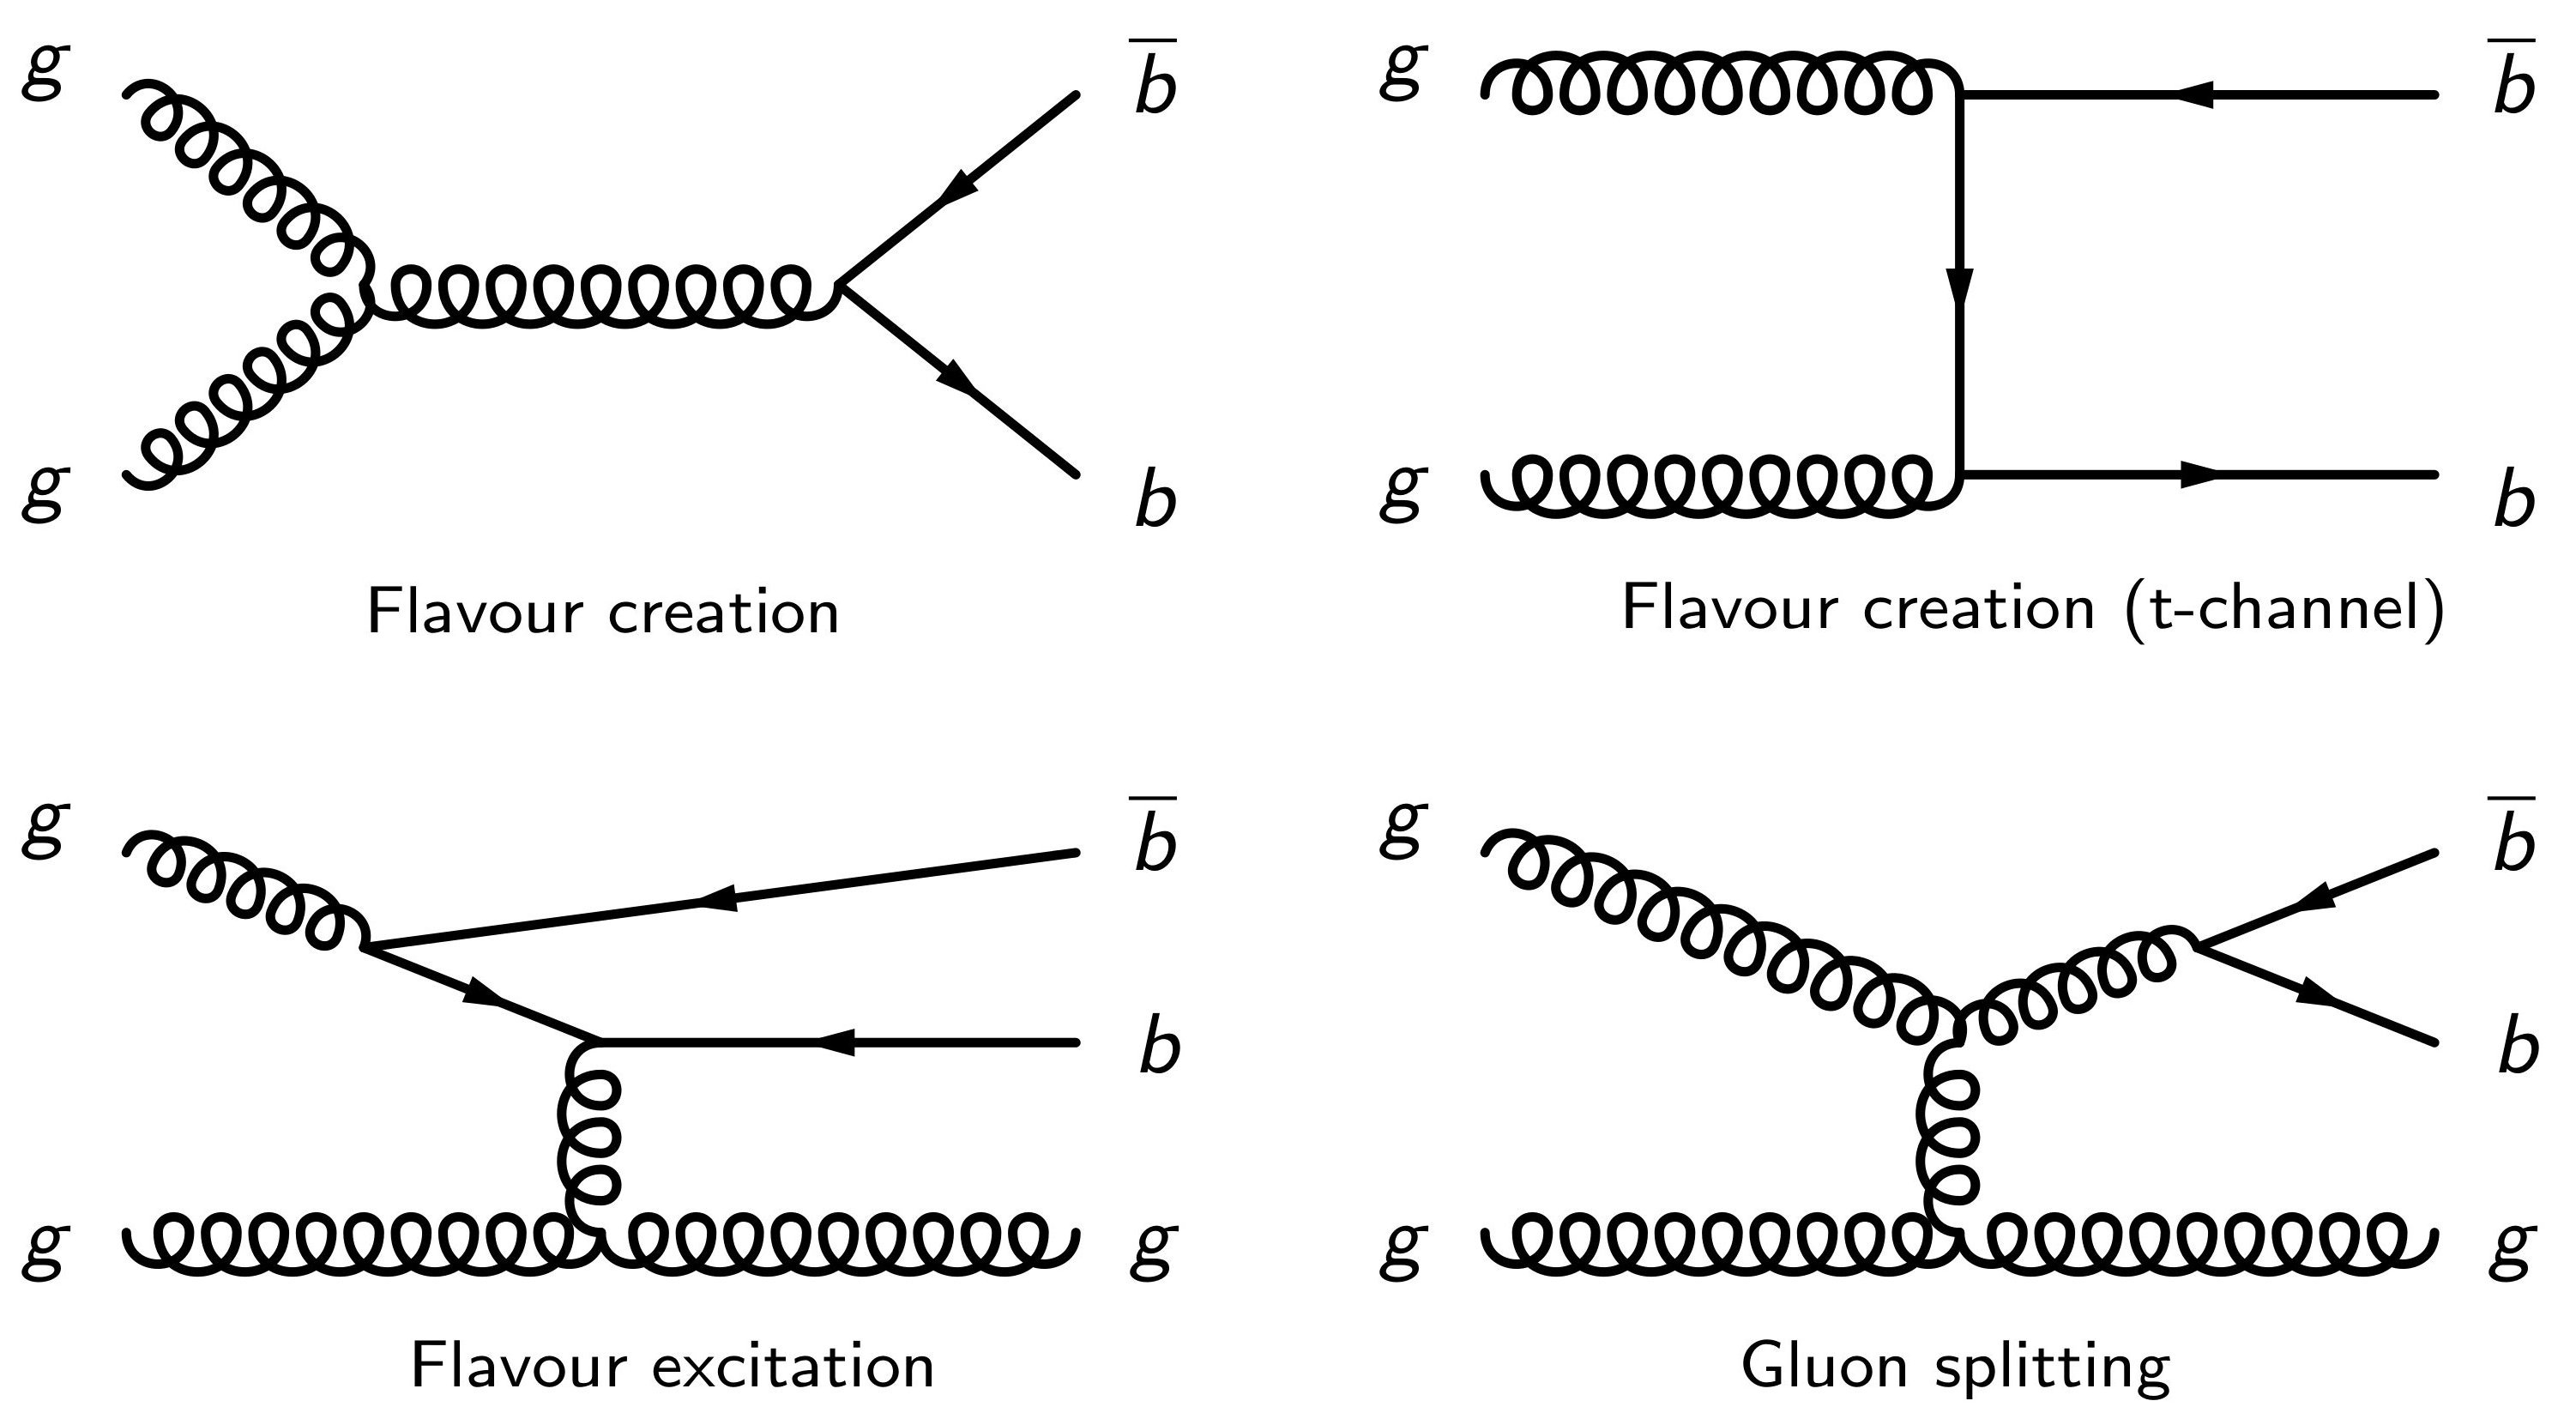
\includegraphics[width=0.32\textwidth,viewport=1600 0 3100 820,clip]{FIGS/bb_diagrams.jpg}
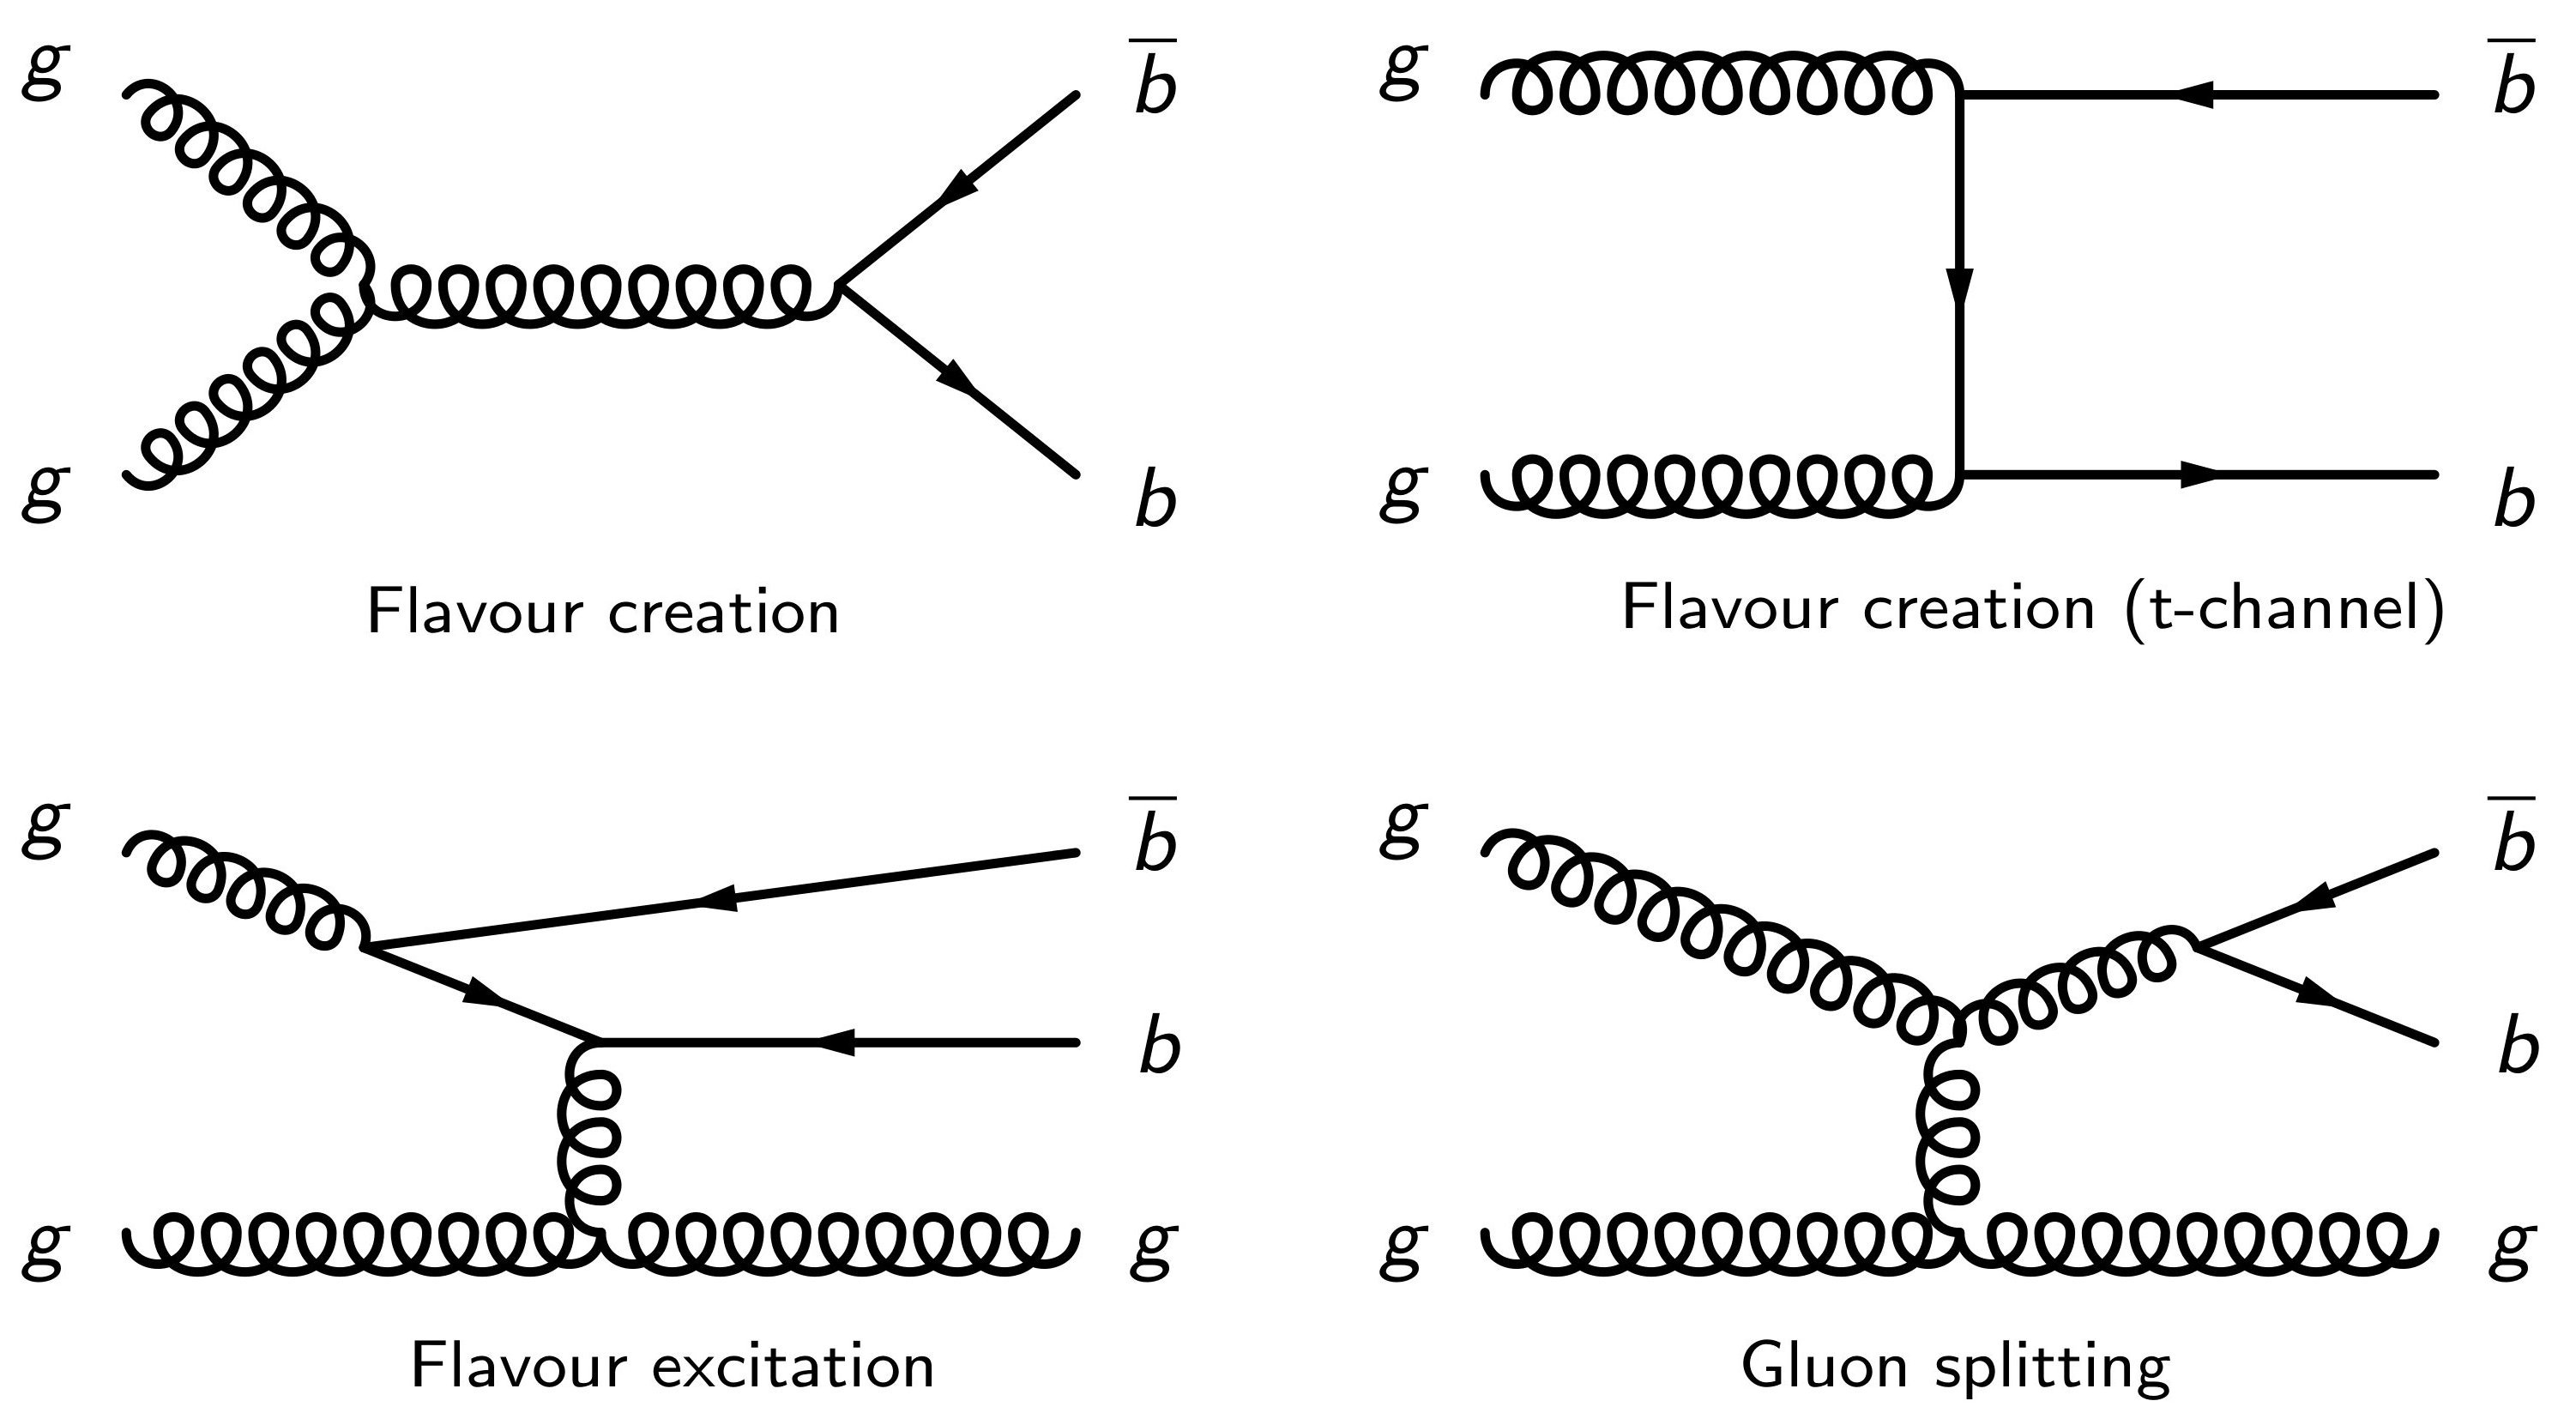
\includegraphics[width=0.32\textwidth,viewport=0 0 1500 820,clip]{FIGS/bb_diagrams.jpg}
\caption{Representative diagrams of the three channels contributing to QCD $b$-quark production up to NLO. The flavour creation channel (left) is the only one present at LO. At NLO, two new channels open up, referred to as gluon splitting (center) and  flavour excitation (right).}
\label{fig:qcd_diagrams}
\end{figure}
%
\\[5mm]
{\em Rejection of background in Standard Model analyses and beyond-SM searches}

Efficient tagging of merged $b$-jets can provide an important handle to understand, estimate and/or reject $b$-tagged backgrounds to SM and new physics searches at the LHC.


%Within the Standard Model (SM) a range of QCD production channels exists for heavy-quark jets, either via pure QCD production or in association with heavy bosons ($W, Z, H$). These channels are expected to produce a mixture of single-$B$ and double $b$-hadron jets. On the other hand, $b$-quarks enter in many collider searches, notably because they are produced in the decays of various SM particles, \eg top quarks, the $Z$ boson and the Higgs boson (if light), and of numerous particles appearing in proposed extensions of the SM. These are expected to produce essentially single-$B$ jets. The ability to distinguish double- from single-$B$ jets is thus of wide application. 

SM physics analyses that rely on the presence of single $b$-jets in the final state, such as top quark physics (either in the $t\bar{t}$ or the single top channels) or associated Higgs production ($WH\rightarrow\ell\nu b\bar{b}$ and $ZH\rightarrow\nu\nu b\bar{b}$),  suffer from backgrounds that can be in part removed by a merged $b$-jet tagger. These are the reducible background from QCD, which can produce double $b$-hadron jets as discussed in the previous subsection, and the irreducible background due to $W$ bosons plus $b$-jets. 
While at LO only single $b$-jets are present in $W+b$ production, at NLO jets containing two $b$-hadrons are expected due to the contribution of diagrams containing a $gb\bar{b}$ vertex.
%One of the leading order diagrams in $W$ + $b$-jets corresponds to $W+g$ followed by $g\to b\bar{b}$ with the $b$-pair produced at small angles and reconstructed as a merged jet. 
The relevance of merged $b$-jets in this channel is supported by NLO calculations of the production of $W$ bosons and two jets with at least one $b$-quark at the LHC~\cite{Campbell:2006}. For jets with $\pt > 25$ GeV, and $|\eta| < 2.5$, they indicate that the cross section for $W(b\bar{b})j$ is almost a factor of two higher than $Wb\bar{b}$, where $(b\bar{b})$ denotes the case in which the two $b$-quarks are merged into the same jet. 

Jets containing a single $b$-quark or antiquark
%Single $b$-jets 
also enter in many BSM collider searches, notably because $b$-quarks are produced in the decays both of heavy SM particles, \eg top quarks, the $Z$ boson and the Higgs boson, and of particles appearing in proposed extensions of the SM. The ability to distinguish single $b$-jets from jets containing two $b$-hadrons is thus here of wide application to reduce SM backgrounds giving rise to close-by $b\bar{b}$ pairs.

%New physics searches with $b$-quarks in the final state also benefit from rejection of QCD and $W+b$ backgrounds which have $b$-jets arising from gluon splitting. 
% TOM % An example is the search for supersymmetry in the framework of generic $R$-parity conserving models~\cite{ATLAS-CONF-2011-098}. The superpartners of quarks and gluons could be copiously produced via the strong interaction at the LHC. The partners of the right- and left-handed quarks, \~{q}$_{L}$ and  \~{q}$_{R}$, can mix to form two mass eigenstates and, since mixing is proportional to the corresponding fermion masses, it becomes more important for the third generation producing sbottom and stop significantly lighter than the other squarks. In this model, thus, sbottom and stop production is expected to dominate. As they chain decay to $b$-quarks and the lightest supersymmetric particle, the signature for this channel is \met\ + (single) $b$-jets. The ability to distinguish single $b$-jets from jets containing two $b$-hadrons is thus here of wide application to reduce SM backgrounds giving rise to merged $b$-jets.
%
%New physics searches with $b$-quarks in the final state also benefit from rejection of QCD and $W+b$ backgrounds which have $b$-jets arising from gluon splitting. An example is the search for supersymmetry in the \met\ + $b$-jets channel~\cite{ATLAS-CONF-2011-098}. Within the framework of a generic $R$-parity conserving models, the superpartners of quarks and gluons are expected to be copiously produced via the strong interaction at the LHC. The partners of the right- and left-handed quarks can mix to form two mass eigenstates and, since mixing is proportional to the corresponding fermion masses, it becomes most important for the third generation producing sbottom ($b_1$) and stop ($t_1$) with masses significantly lighter than those of the other squarks. In this model, thus, sbottom and stop production is expected to dominate, and they chain decay to $b$-quarks and the lightest supersymmetric particle, with a \met\ + $b$-jets signature.
%
% TOM % \\[5mm]
% TOM % {\em Study of jet substructure and boosted objects}
% TOM % 
% TOM % At the LHC, many of the particles considered to be heavy at previous accelerators will be frequently produced with a transverse momentum greatly exceeding their rest mass, like the electro-weak gauge bosons $W^\pm$ and $Z$, the top quark, the Higgs boson (or bosons) and possibly other new particles in the same mass range. These boosted objects, produced either by recoil against other energetic objects or from decays of even heavier BSM particles, upon decay can give rise to a highly collimated topology too close to be resolved by standard jet algorithms. For theses cases, sophisticated tools have been developed in the last years~\cite{boost2010,boost2010b} to analyse the substructure of the ensuing jet and reveal its heavy-particle origin.
% TOM % 
% TOM % The analysis of double $b$-hadron jets is an ideal testbed for studying jet substructure in data, as it provides a large supply of boosted, merged jets. Within the framework of a  %LO 
% TOM % parton-shower Monte Carlo generator, double $b$-hadron jets largely originate from gluon splitting into two $b$-quarks whose angular separation is comparable or smaller than the size parameter of the jet algorithm. For instance, for a dijet QCD sample generated with {\sc Pythia6} (see details in section~\ref{sec:Simulation}), the fraction of merged $b$-jets from gluon splitting is 94\% (97\%) for jets with $\pt=60$~GeV ($\pt=300$~GeV) reconstructed with the anti-$k_t$ algoritm and size parameter $R=0.4$. The understanding of the substructure of these jets is also important as they are themselves the background to boosted object searches, like $Z\rightarrow b\bar{b}$ or $H\rightarrow b \bar{b}$.  
%In particular, it has recently been suggested~\cite{Butterworth:2008iy} that $WH$ and $ZH$ production can become potential discovery and analysis channels by restricting one's attention to the $\sim5$\% of events in which the vector and Higgs bosons have large transverse momentum, ${\pt}_H\gtrsim200$ GeV. Understanding the much more common QCD events with $b\bar{b}$ jets will be essential before attempting to measure these rare final states.






%%%%%%%%%%%%%%%%%%%%%%%%%%%%%%%%%%%%%%%%%%%%%%%%%%%%%%%%%%%%%%%%%%%%%%%%%
%  Gluon splitting fraction in hadronic Z decays (SLD, DELPHI)
%%%%%%%%%%%%%%%%%%%%%%%%%%%%%%%%%%%%%%%%%%%%%%%%%%%%%%%%%%%%%%%%%%%%%%%5%


The average multiplicity of $b\bar{b}$ pairs from gluons in hadronic $Z^0$ decays was first measured by DELPHI experiment at LEP. The analysis was performed by looking for secondary vertex production in 4-jet events. The average rate was found to be (0.21$\pm$0.11(stat.)$\pm$0.09(syst.))\%~\cite{Abreu:1997nf}.

The rate of gluon splitting into bottom quarks, $g \rightarrow b\bar{b}$, was also measured by the Stanford Linear Collider (SLC) Large Detector (SLD), in hadronic $Z^0$ decays collected from 1996 to 1998~\cite{Abe:1999vw}. Following a similar procedure, the rate per hadronic event was found to be (3.7$\pm$0.71(stat.)$\pm$0.66(syst.))$\times$10$^{-3}$. %In order to improve singal/background ratio, topological information was used. A cut on $cos\theta$ between the two most energetic jets, jets 1 and 2 is performed to remove $b\bar{b}$ background with one $b$-jet splitting into two giving rise to two very collinear vertex axis.  Secondly, the variable $|cos\alpha_{1234}|$, where $alpha_{1234}$ is the angle between the plan formed by jets 1 and 2 and the plane formed by jets 3 and 4, is used to supress the $b\bar{b}$ background. This variable is useful to separate $g\rightarrowb\bar{b}$ events because the radiated virtual gluon in the process $Z^0 \rightarrow q\bar{q}g $ is polarized in the plane of the three-parton event, and this is reflected in the subsequent splitting, by strongly favoring $g\rightarrowb\bar{b}$ emission out of this plane.

 The probability for secondary production of a bottom quark pair from a gluon per hadronic $Z^0$ decay in $e^+e^-$ annihilation, 
\begin{equation} 
g_{b\bar{b}} = \frac{N(Z^0 \rightarrow q\bar{q}g,g\rightarrowb\bar{b} )}{N(Z^0\rightarrow hadrons)}
\end{equation} 
is expected to be very small, since the gluon must have sufficient energy to produce the bottom quark pair. 

 At the Tevatron, on the other hand, 50\% of the $B$
 hadrons are due to the gluon splitting process, and a larger fraction is expected to contribute at the LHC.




%%%%%%%%%%%%%%%%%%%%%%%%%%%%%%%%%%%%%%%%%%%%%%%%%%%%%%%%%%%%%%%%%%%
%  Our work, plus content
%%%%%%%%%%%%%%%%%%%%%%%%%%%%%%%%%%%%%%%%%%%%%%%%%%%%%%%%%%%%%%%%%%%




\\[5mm]
There are two possible strategies to attempt to identify $b$-jets containing two $b$-hadrons in hadronic collisions. One of them relies on the direct reconstruction of the two $b$-decay secondary vertices~\cite{CDFAzimutalCorrelation}. This %has the further advantage of allowing 
allows the measurement of the angular separation between the $b$-hadrons, but suffers from the low efficiency of a double $b$-tag requirement plus additional reconstruction inefficiencies at small angular separation between the two $b$-hadrons. In this thesis we develop an alternative method that does not rely on explicit vertex finding, but exploits the substructure differences between single and merged $b$-jets, combining them in a multivariate analysis. 

Chapter~\ref{ch:theory} describes the theoretical framework, with emphasis in the theory of the strong interactions and the aspects that are important for the understanding of the hadronic final state in hadronic collisions. The LHC and the ATLAS detector components  are described in Chapter~\ref{ch:lhc_atlas}, together with a summarization of the detector conditions during 2011 data taking.  Chapter~\ref{ch:reco} details how jet reconstruction and calibration are performed at ATLAS and describes the procedure for the identification of $b$-quark jets. Chapter~\ref{ch:kinematic} presents the analysis of jet shape and substructure variables for the discrimination between single and double $b$-hadron jets. The validation of the variables in 2011 data is also included.   The construction of the multivariate discriminator  and the discussion of the systematic uncertainties are presented in Chapter~\ref{ch:mva}. 

{\sc To do}
Preliminary results for the measurement of the fraction of double $b$-hadron jets in data are discussed in Chapter~\ref{ch:gbbfraction}. 

Finally, chapter~\ref{ch:conclusions} summarizes the results. 




